\section{Vorwort}
Bei der Recherche zur Bearbeitung des Projektes wurden viele englische Webseiten zu rate gezogen. Viele englische Fachbegriffe haben sich im Bereich Software durchgesetzt, so dass 
eine Übersetzung eher verwirren als helfen würde. Die \textbf{englischen} Bezeichner und Beschreibungen von Flags und Optionen wurde beibehalten, da diese auch in den man-pages Verwendung finden und in Internet-Foren vorrangig anzutreffen sind.

\section{Projektbeschreibung}
Das erklärte Ziel der pi4\_robotics GmbH Berlin ist es humanoide Roboter zu entwickeln. 
Diese können bereits in unterschiedlichen Branchen eingesetzt werden. Im Werbeblatt 
des Workerbot4 (siehe Anhang, Kapitel 13) werden die Basisfähigkeiten des Jolandi Workerbot beschrieben.  \\
Bisher ist das Anlernen neuer Tätigkeiten und die Bedienung nur über eine PC-Schnittstelle möglich, doch das soll sich ändern. Es ist geplant Spracherkennung und visuelle Wahrnehmung 
zu integrieren. Um mit dem Roboter wie mit einem Menschen kommunizieren zu können. Auch soll 
ein Avatar Modus implementiert werden, bei dem der User in die Rolle des Roboters schlüpft 
und per Teleoperation den Roboter bewegt, hört was der Roboter hört und mit den Augen des Roboters sieht. \\
Für den Einsatz als Sicherheitspersonal ist weiterhin geplant, die Stimme des Bedieners aus dem Roboter Lautsprecher ertönen zu lassen und sein Gesicht auf dem Kopfdisplay anzuzeigen. 
Der Kunde soll das Gefühl haben, dass der Roboter der Avatar des Bedieners ist.\\
Für die Laborübungen 'Entwurf eingebetteter Systeme' und 'Netzwerk-Programmierung' wurde 
bidirektionale Ton und Video Übertragung ausgewählt. Dabei galt es Audio und Video 
\textbf{mehrerer} Roboter auf eine Webseite zu streamen und eine Webcam inklusive Ton des PC 
auf alle verbundenen Roboter zurück zu streamen.\\
\begin{minipage}{\textwidth}
    \begin{center}
        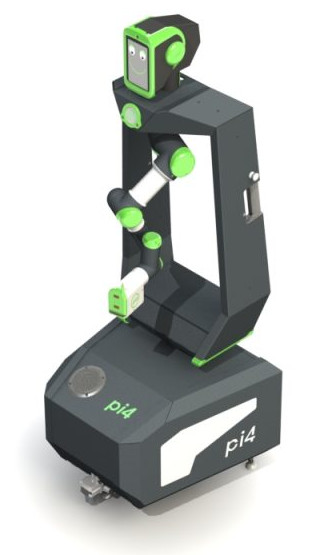
\includegraphics[scale=0.5]{img/jolandi.jpg} 
    \end{center}
\end{minipage}
\begin{center}
Jolandi Workerbot der Firma pi4\_robotics GmbH
\end{center}
 
\begin{minipage}{\textwidth}
    \begin{center}        
        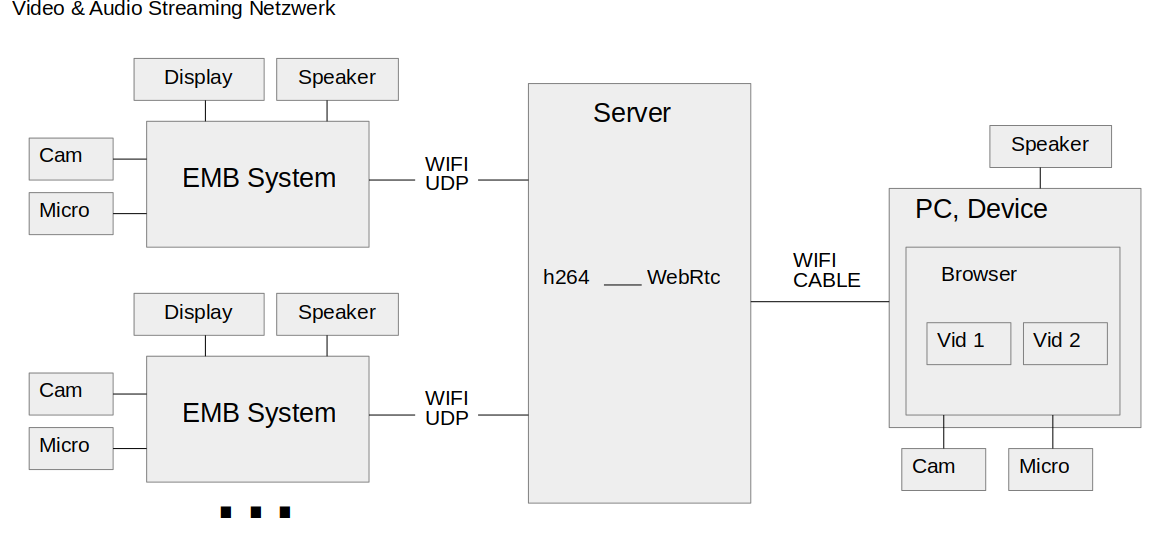
\includegraphics[scale=0.4]{img/schemaproj.png} 
    \end{center}
\end{minipage}
\begin{center}
Schemaplan der Komponenten
\end{center}
Links auf dem Schemaplan sind die in Robotern integrierten eingebettete Systeme gezeigt. Pro Roboterkopf ist ein Raspberry PI mit Touch-Display verbaut. Für das Projekt wurde jeweils eine Webcam für Ton und Video angeschlossen. Die Tonwiedergabe erfolgt über einen USB Lautsprecher. \\
Auf der rechten Seite des Plans ist der Bediener PC dargestellt. Auch hier liefert eine Webcam Ton und Video. Ton wird über die PC Lautsprecher ausgegeben.\\
Für den Bediener soll ein Web-Template erstellt werden. Dort kann ausgewählt werden, welcher Videostreams angezeigt werden soll. Der Zeitversatz bei der Übertragung soll sehr gering sein 
(<0.2sec), damit der User möglichst schnell reagieren kann. Bildübertragung zum eingebetteten System darf einen leichten Zeitversatz haben, da dort nur das Gesicht des Bedieners angezeigt wird, aber keine weiteren Handlungen davon abhängen.\\
Das gesamte Streaming soll über das Internet erfolgen. Dabei ist der Datentransfer auch aus 
fremden WLAN Netzen heraus zu realisieren. Fremd im Sinne, dass die dazwischen liegende Router und Ports nicht konfigurierten werden können. Die IP Adressen der Roboter sind damit quasi unbekannt, d.h. dynamisch wechselnd und nicht vom Internet aus sichtbar.\\
 

\subsection{Streaming Basis Komponenten}
Streaming live convent over the internet requires much more extra care than just providing web page content since a downtime in the service can significantly affect the image of the company and cause it to lose content consumers and advertisers. There are several services on the internet that provide services to reliably stream audio and video content over the internet. However these paid services can be very expensive due to the importance of the availability of the service. Nevertheless, there is a cheaper alternative which is secure and reliable at the same time to set up an audio and/or video stream service on your own.

Any streaming service requires 3 components in order to work: a streaming server, a stream source and a client.

\textbf{Streaming server:}  This is the main component that passes (and sometimes re-encode) the audio and/or video content from each of the sources to the connected audience. There are several streaming servers both proprietary and open source that can be used. Among the open source alternatives, the most popular are Shoutcast and Icecast, both are easy to install and have proved to be very reliable and secure. To provide a single streaming point Shoutcast is the preferred option, however, to provide a more flexible service that allows multiple sources (different bitrates for example) Icecast might be more suitable. The advantage of Icecast over Shoutcast is that it introduces the concept of mountpoints which are independent streams mounted over the same server which distributes the resources efficiently among all the mountpoints. A Shoutcast example will be shown in this case.\\
\textbf{Stream Source:} A source provides the audio and/or video content to the streaming server. It usually provides capabilities to manage playlists and re-encode audio/video content. It does not need to be on the same physical server as the streaming server but it is recommended to be on a different server. A plugin for Winamp can be used as a source for a Shoutcast server which basically will send any content played on Winamp to a Shoutcast stream server. Liquidsoap is very powerful and programmable streaming source that allows generating a reliable streaming with fallback options. Liquidsoap can be used with either Icecast or Shoutcast. In addition, Liquidsoap provides a very strong a powerful API that allows generating different playlists, introducing jingles and defining fallback sources to produce a continuous streaming in case the main source becomes unavailable. Fallback is also available at server level in Icecast to provide an even more reliable streaming. The liquidsoap API also provides DSP (Digital Signal Processing) capabilities that allow programmatically mixing tracks, normalizing and controlling volume, and even introducing some effects. In this example, A simple Liquisoap script will be shown\\
\textbf{Client:} A client is referred to the software being used by the consumer to playback the stream.  This can vary greatly and depends on the preference of each user, but most of the current players (WMP, Quicktime, Winamp, iTunes, etc) will be able to playback audio streams in mp3 and other widely used formats. Some players provide plug-ins so streams can be played directly from the web browser. Other common formats in audio streams are aac+, asf, and ogg.




